\begin{figure}[htbp]
\centering
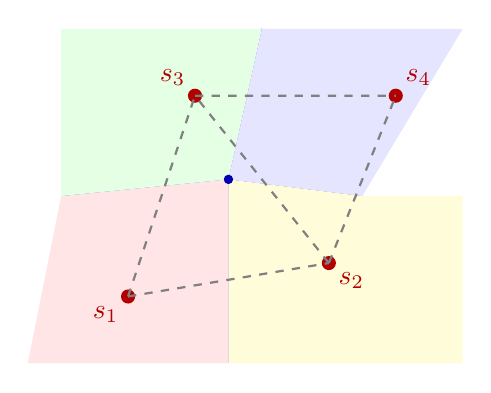
\begin{tikzpicture}[scale=0.85]
  \coordinate (s1) at (0,0);
  \coordinate (s2) at (3,0.5);
  \coordinate (s3) at (1,3);
  \coordinate (s4) at (4,3);
  \draw[blue!60,thick] (-1,1.5)--(1.5,1.75)--(3.5,1.5);
  \draw[blue!60,thick] (1.5,1.75)--(2,4);
  \draw[blue!60,thick] (1.5,1.75)--(1.5,-1);
  \fill[red!10] (-1.5,-1)--(-1,1.5)--(1.5,1.75)--(1.5,-1)--cycle;
  \fill[green!10] (1.5,1.75)--(-1,1.5)--(-1,4)--(2,4)--cycle;
  \fill[blue!10] (1.5,1.75)--(2,4)--(5,4)--(3.5,1.5)--cycle;
  \fill[yellow!15] (1.5,1.75)--(3.5,1.5)--(5,1.5)--(5,-1)--(1.5,-1)--cycle;
  \fill[red!70!black] (s1) circle (3pt) node[below left] {$s_1$};
  \fill[red!70!black] (s2) circle (3pt) node[below right] {$s_2$};
  \fill[red!70!black] (s3) circle (3pt) node[above left] {$s_3$};
  \fill[red!70!black] (s4) circle (3pt) node[above right] {$s_4$};
  \draw[gray,dashed,thick] (s1)--(s2) (s1)--(s3) (s2)--(s3) (s2)--(s4) (s3)--(s4);
  \fill[blue!70!black] (1.5,1.75) circle (2pt);
\end{tikzpicture}
\caption{Voronoi diagram (colored cells) and its Delaunay triangulation dual (dashed gray edges). Each Voronoi vertex is the circumcenter of a Delaunay triangle.}
\label{fig:voronoi_duality}
\end{figure}
